

\documentclass[journal,12pt,twocolumn]{IEEEtran}
\usepackage[none]{hyphenat}
\usepackage{enumitem}
\usepackage{graphicx}
\usepackage{listings}
\usepackage{kvmap}
\usepackage[english]{babel}
\usepackage{graphicx}
\usepackage{caption} 
\usepackage{tikz}
\usepackage{hyperref}
\usetikzlibrary{arrows,shapes,automata,petri,positioning,calc}
\usepackage{multirow}


\title{Assignment \textrm{I}
\textbf{\\Design of  non overlapping sequence detector}}
\author{sireesha abbavaram - FWC22060}
\date{\today}
\begin{document}
\maketitle

\tableofcontents 
\vspace{0.5cm}

\begin{abstract}
This manual shows how to design a sequential circuit for non overlapping sequence of110011.
\end{abstract}

\section{Components}
\begin{tabular}{|c|c|c|}
\hline
Components & Value & Quantity\\
\hline
Resistor & 220 Ohm & 1\\
\hline
Arduino & UNO & 1\\
\hline
Seven Segment Display & & 1\\
\hline
Decoder & 7447 & 1\\
\hline
Flip Flop & 7474 & 2\\
\hline
Bread Board & & 1\\
\hline
Jumper Wires & & 20\\
\hline
\end{tabular}

\section{Hardware}
\begin{enumerate}
\item Make connections between the seven segment display in Fig 1 and the 7447 IC in Fig 2 as shown in Table \ref{table:1}
\item Connect the Arduino, 7447 IC and the two 7474 ICs according to Table 2 and Fig 3.
\item Input is given from Arduino D8.
\vspace{0.5cm}
\end{enumerate} 

\begin{figure}[h!]
\centering
\includegraphics[height=8cm,width=4cm]{display.png}
\centering
\caption{Seven Segment Display}
\end{figure}


\begin{table}[h]
\Large
\centering
\begin{tabular}{|c|c|c|c|c|c|c|c|}
\hline
7447 & a' & b' & c' & d' & e' & f' & g'\\
\hline
Display & a & b & c & d & e & f & g\\
\hline
\end{tabular}
\caption{Connection Table}
\label{table:1}
\end{table}

\section{Finite State Machine}
\begin{enumerate}
\item A sequential detector is a sequential state machine that takes an input string of bits and generates an output 1 whenever the target sequence has been detected.
\item The Input is changed to 0 and 1 to display the Next state.
\item The LED glows when the sequence 110011 is detected.
\end{enumerate} 


\begin{figure}[h!]
\centering
\includegraphics[width=8cm, height=4cm]{7447.png} 
\centering
\caption{Pin Diagram of 7447 IC}
\end{figure}

\begin{figure}[h!]
\centering
\includegraphics[width=8cm, height=4cm]{7474.png}
\centering
\caption{Pin Diagram of 7474 IC}
\end{figure}

\begin{figure}

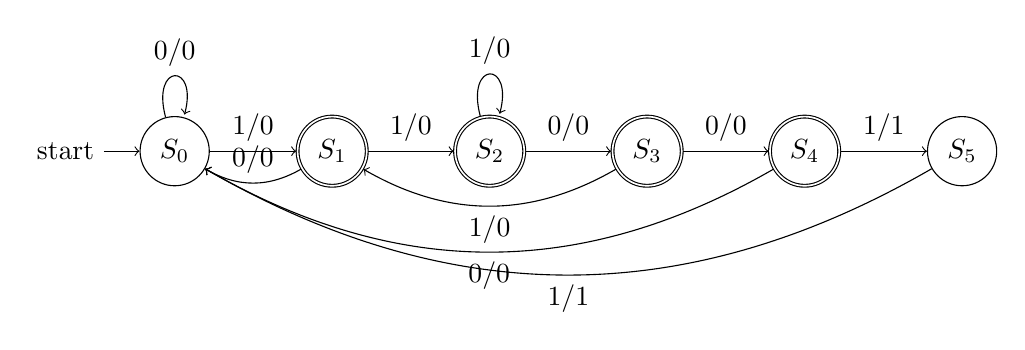
\begin{tikzpicture} [node distance=2cm]
\node[circle, draw, state, initial] (S0) {$S_0$};
\node[circle, draw, state, accepting, right of=S0] (S1) {$S_1$};
\node[circle, draw, state, accepting, right of=S1] (S2) {$S_2$};
\node[circle, draw, state,accepting, right of=S2] (S3) {$S_3$};
\node[circle,draw,state,accepting,right of=S3] (S4) {$S_4$};
\node[circle,draw,state,right of=S4] (S5) {$S_5$};
\path[->] (S0) edge[above] node{1/0} (S1)
          (S1) edge[above] node{1/0} (S2)
          (S2) edge[above] node{0/0} (S3)
          (S3) edge[above] node{0/0} (S4)
          (S4) edge[above] node{1/1} (S5)
          (S0) edge[loop above] node{0/0} (S0)
          (S1) edge[above,bend left] node{0/0} (S0)
          (S2) edge[loop above] node{1/0} (S2)
          (S3) edge[below,bend left] node{1/0} (S1)
          (S4) edge[below,bend left] node{0/0} (S0)
          (S5) edge[below,bend left]
node{1/1} (S0);
         
\end{tikzpicture}
\caption{State Diagram}
\end{figure}

\centering
\begin{table}[h!]
\large
\begin{tabular}{|l|ll|llll|cl|clll|}
\hline
\multirow{2}{*}{} & \multicolumn{2}{c|}{INPUT}   & \multicolumn{4}{c|}{OUTPUT}                                                      & \multicolumn{2}{c|}{\multirow{2}{*}{CLOCK}} & \multicolumn{4}{c|}{\multirow{3}{*}{5V}}                                       \\ \cline{2-7}
                  & \multicolumn{1}{l|}{P}   & Q  &  \multicolumn{1}{l|}{D}  & \multicolumn{1}{l|}{C}  & \multicolumn{1}{l|}{B}  & A  & \multicolumn{2}{c|}{}                       & \multicolumn{4}{c|}{}                                                          \\ \cline{1-9}
Arduino           & \multicolumn{1}{l|}{D6} & D7 & \multicolumn{1}{l|}{D10} & \multicolumn{1}{l|}{D11} & \multicolumn{1}{l|}{D4} & D5 & \multicolumn{2}{c|}{D13}                    & \multicolumn{4}{c|}{}                                                          \\ \hline
7474              & \multicolumn{1}{l|}{2}  & 12 & \multicolumn{1}{l|}{}   & \multicolumn{1}{l|}{}   & \multicolumn{1}{l|}{9}  & 5  & \multicolumn{1}{l|}{CLK1}       & CLK2      & \multicolumn{1}{l|}{1} & \multicolumn{1}{l|}{4} & \multicolumn{1}{l|}{10} & 13 \\ \hline
7474              & \multicolumn{1}{l|}{}  &  & \multicolumn{1}{l|}{5}   &  \multicolumn{1}{l|}{2}   & \multicolumn{1}{l|}{}  &    & \multicolumn{1}{l|}{CLK1}       & CLK2      & \multicolumn{1}{l|}{1} & \multicolumn{1}{l|}{4} & \multicolumn{1}{l|}{10} & 13 \\ \hline
7447              & \multicolumn{1}{l|}{}   &    & \multicolumn{1}{l|}{}   & \multicolumn{1}{l|}{}   & \multicolumn{1}{l|}{1}  & 7  & \multicolumn{1}{l|}{}           &           & \multicolumn{4}{c|}{16}                                                        \\ \hline
\end{tabular}
\centering
\caption{Connection Table}
\label{table:2}
\end{table}

\begin{table}[h!]
\begin{tabular}{|c|c|c|c|}
\hline
\textbf Present State & Input & Next State & Output \\
\hline
\textbf A B C & X & P Q R & Y\\
\hline
0 0 0 & 0 & 0 0 0 & 0\\
0 0 0 & 1 & 0 0 1 & 0\\
0 0 1 & 0 & 0 0 0 & 0\\
0 0 1 & 1 & 0 1 0 & 0\\
0 1 0 & 0 & 0 1 1 & 0\\
0 1 0 & 1 & 0 1 0 & 0\\
0 1 1 & 0 & 1 0 0 & 0\\
0 1 1 & 1 & 0 0 1 & 0\\
1 0 0 & 0 & 0 0 0 & 0\\
1 0 0 & 1 & 1 0 1 & 0\\
1 0 1 & 0 & 0 0 0 & 0\\
1 0 1 & 1 & 0 0 0 & 1\\
\hline
\end{tabular}
\centering
\caption{State Table}
\label{table:2}
\end{table}
\hspace{2cm}
\begin{kvmap}
    \begin{kvmatrix}{Q,R,P,X}
    0 & 0 & 1 & 0\\
    0 & 0 & X & X\\
    1 & 0 & X & X\\
    0 & 0 & 0 & 0\\
    \end{kvmatrix}
    \bundle[color=red]{2}{0}{2}{0}
    \bundle[color=blue]{0}{2}{0}{2} 
\end{kvmap}


\begin{equation}
A=X'P'QR+XPQ'R'
\label{eq1}
\end{equation}
  
\hspace{2cm}
\begin{kvmap}
    \begin{kvmatrix}{Q,R,P,X}
    0 & 0 & 0 & 1\\
    0 & 0 & X & X\\
    0 & 0 & X & X\\
    0 & 1 & 0 & 1\\
    \end{kvmatrix}
    \bundle[color=red]{3}{0}{3}{3}
    \bundle[color=blue]{1}{3}{1}{3}
\end{kvmap}
\begin{equation}
    B=P'QR'+XP'Q'R
\label{eq1}
\end{equation} 
 
\vspace{6cm}
\begin{kvmap}
    \begin{kvmatrix}{Q,R,P,X}
    0 & 0 & 0 & 1\\
    0 & 0 & X & X\\
    1 & 0 & x & x\\
    1 & 0 & 1 & 0\\
    \end{kvmatrix}
    \bundle[color=red]{3}{0}{3}{0}
    \bundle[color=blue]{2}{3}{2}{3}
    \bundle[color=green]{0}{2}{0}{3}
    
\end{kvmap}
\begin{equation}
C=XQ'R'+XP'QR+X'P'QR'
\label{eq1}
\end{equation}  

\begin{equation}
D=XPQ'R
\label{eq1}
\end{equation}

\vspace{6cm}
\section*{Conclusion}
The detection of 110011 sequence  is implemented using
\begin{table}[h]
\large
\centering
\begin{tabular}{|l|}
\hline

https://github.com/sireesha1602/sireesha/
\\blob/main/ide/code.cpp \\

\hline
\end{tabular}

\end{table}
\end{document}
